\documentclass[]{article}

\usepackage{graphicx}
\usepackage{lmodern}
\usepackage{amssymb,amsmath}
\usepackage{ifxetex,ifluatex}
\usepackage{fixltx2e} % provides \textsubscript
\ifnum 0\ifxetex 1\fi\ifluatex 1\fi=0 % if pdftex
  \usepackage[T1]{fontenc}
  \usepackage[utf8]{inputenc}
\else % if luatex or xelatex
  \ifxetex
    \usepackage{mathspec}
  \else
    \usepackage{fontspec}
  \fi
  \defaultfontfeatures{Ligatures=TeX,Scale=MatchLowercase}
\fi
% use upquote if available, for straight quotes in verbatim environments
\IfFileExists{upquote.sty}{\usepackage{upquote}}{}
% use microtype if available
\IfFileExists{microtype.sty}{%
\usepackage{microtype}
\UseMicrotypeSet[protrusion]{basicmath} % disable protrusion for tt fonts
}{}
\usepackage[unicode=true]{hyperref}
\hypersetup{
            pdfborder={0 0 0},
            breaklinks=true}
\urlstyle{same}  % don't use monospace font for urls
\IfFileExists{parskip.sty}{%
\usepackage{parskip}
}{% else
\setlength{\parindent}{0pt}
\setlength{\parskip}{6pt plus 2pt minus 1pt}
}
\setlength{\emergencystretch}{3em}  % prevent overfull lines
\providecommand{\tightlist}{%
  \setlength{\itemsep}{0pt}\setlength{\parskip}{0pt}}
\setcounter{secnumdepth}{0}
% Redefines (sub)paragraphs to behave more like sections
\ifx\paragraph\undefined\else
\let\oldparagraph\paragraph
\renewcommand{\paragraph}[1]{\oldparagraph{#1}\mbox{}}
\fi
\ifx\subparagraph\undefined\else
\let\oldsubparagraph\subparagraph
\renewcommand{\subparagraph}[1]{\oldsubparagraph{#1}\mbox{}}
\fi

\title{Windowless percentile tracking}
\author{Martin Jambon\\
        \texttt{martin@mjambon.com}}
\date{July 23, 2016\\
Last revised July 1, 2017}

\begin{document}
\maketitle

\begin{abstract}
This is a method driven by the same constraints as the exponential
moving average, but for median and other percentiles.

We present an algorithm for tracking the value of a percentile, such as
the median, in an infinite stream of observations whose distribution can
change over time. A self-imposed constraint is that we cannot afford to
keep the last \emph{N} observations explicitly in memory, even for
modest values of $N$ such as 100.
Our solution involves a single parameter denoted \(r\)
that expresses the trade-off between accuracy and reactivity
to changes in the distribution of the signal.
The cost of updating the estimated percentile is constant in
time and space, and is independent of $r$.
\end{abstract}

Notations: in this document, all sequences and arrays are indexed
starting from~0.

\subsection{Background: window-based
algorithms}\label{background-window-based-algorithms}

Given \emph{N} a fixed window length, it is relatively straightforward
to maintain a sorted array \(W\) of the latest \emph{N} observations
indexed \(0\dots N-1\). The \emph{p}-percentile is computed exactly over
that window by looking up the pair of values found at index
\(\lfloor (N-1)p \rfloor\) and at index \(\lceil (N-1)p \rceil\), and by
taking their average.

For example, the median \(m\) (0.5-percentile) using a window of length
\(N=100\) is calculated as follows once we've read 100 observations or
more:

\[m = \frac{W_{49} + W_{50}}{2}\]

Such algorithms are not acceptable for us since they require storing the
latest \emph{N} values, where \emph{N} is typically chosen greater than
100.

\subsection{Background: exponential moving
average}\label{background-exponential-moving-average}

An exponential moving average is a weighted average of the previous
observations, in which the weight of the latest observation is always
set to a fixed parameter \(r\) (\(0 < r \le 1\)) and the weight of the
other values is \((1-r)\) times their previous weight.

After reading \(\lfloor 1/r \rfloor + 1\) observations or more, the
moving average for observation \emph{i} is computed as follows:

\[m_i = r . x_i + (1-r) . m_{i-1}\]

In the initial phase where \(i < \lfloor 1/r \rfloor\), \(m_i\) is
calculated as the mean of all the observations so far. The rationale is
that the weight of the latest observation is the nearest possible to
\(r\) without being smaller than the weight any of the past
observations. This avoids having to set \(m_{-1}\) to an arbitrary guess
with a lasting impact. Updating \emph{m} in this initial phase is done
as follows:

\[\hat{r}_i = \frac{1}{i+1}\]
\[m_i = \hat{r}_i . x_i + (1-\hat{r}_i) . m_{i-1}\]

This exponential moving average algorithm is used in the moving
percentile algorithm described below to estimate the standard deviation
of the signal.

\subsection{Moving percentile
algorithm}\label{moving-percentile-algorithm}

The \(p\)-percentile is represented by the variable \(m\). It is
initialized with the value of the first observation \(x_0\):

\[ m_0 = x_0 \]

Subsequent iterations are updated as follows, for some value of
\(\delta\) discussed later.

If \(x_i < m_{i-1}\) then

\[ m_i = m_{i-1} - \frac{\delta}{p} \]

else if \(x_i > m_{i-1}\) then

\[ m_i = m_{i-1} + \frac{\delta}{1-p} \]

else \(x_i = m_{i-1}\) and keep the previous value:

\[ m_i = m_{i-1} \]

If \(\delta\) is not too large and not too small, \(m\) is a good
estimate of the \(p\)-percentile. Choosing a good value for \(\delta\)
depends on the distribution of values around the \(p\)-percentile.
Excessive values of \(\delta\) result in big jumps for \emph{m} and
limit the accuracy, while a \(\delta\) that's too small may take too
much time to converge to the \(p\)-percentile as computed exactly using
a window of a reasonable length.

In order to express the trade-off between accuracy and convergence
speed, we express \(\delta\) as the product of a user-chosen constant
\emph{r} and the estimated standard deviation \(\sigma\) of the input
signal:

\[ \delta_i = \sigma_i . r \]

where \(\sigma_i\) is the square root of the variance estimated by a
moving average of the sequence
$\{ \dots, (\mu_{i-1} - x_{i-1})^2, (\mu_i - x_i)^2 \}$, where
\(\mu_i\) itself is a moving average of the sequence
$\{ \dots, x_{i-1}, x_i \}$.

We find that reasonable values of \(r\) for many applications range from
0.001 to 0.01.

\clearpage

The chart below shows our sample signal that was generated randomly in 3
phases:

\begin{itemize}
\tightlist
\item
  phase 1 (0-999): Uniform(0,1); expected 0.9-percentile = 0.9
\item
  phase 2 (1000-1999): Uniform(2,4); expected 0.9-percentile = 3.8
\item
  phase 3 (2000-2999): Uniform(0,1); expected 0.9-percentile = 0.9
\end{itemize}

The output for window-based percentile estimators and for our moving
percentile are shown here:

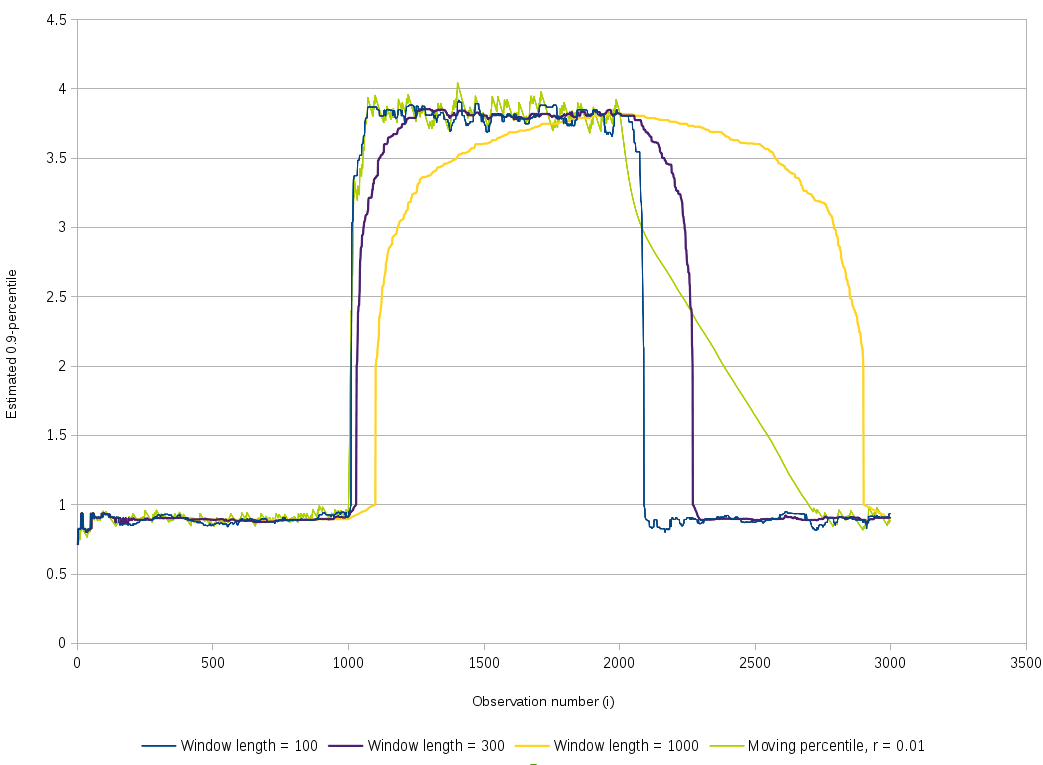
\includegraphics[width=\textwidth]{img/moving-percentile-output}

Our moving 0.9-percentile, shown on the chart in green, reacts quickly
when the signal shifts upward, because each update shifts the moving
percentile upward by \(\frac{\delta}{0.1}\). However, when the signal
shifts downward, it takes the moving percentile more time to react
because each update shifts it downward by \(\frac{\delta}{0.9}\), which
is 9 times less than in the other direction. Additionally, we can see
that the downward shift is pretty steep initially and then gets less
steep. This is due to the delayed update of the standard deviation
\(\sigma\): the value of \(\delta\) is divided by two when the estimated
\(\sigma\) catches up and is divided by two, reflecting the new
distribution in phase 3.

A sample implementation is provided on GitHub at \\
\verb|https://github.com/mjambon/moving-percentile|.

\end{document}
